% !TEX root = Dissertation-vLautz.tex

\documentclass[a4paper,
               11pt,
               twoside,
               parskip=half,
               headings=big]{scrbook}

\usepackage{microtype} % enable typographic optimisations

% === Linespacing
% space between paragraphs instead of firstline indent
% to avoid unsightly vertical spacing enable ragged raggedbottom
% this means bottom line on opposing pages won't line up, but so it goes
\usepackage[onehalfspacing]{setspace}
\raggedbottom
% set binding correction and DIV after setspace
\KOMAoptions{BCOR=14mm, DIV=13}%12
% set headings to singlespacing
\setkomafont{chapter}{\singlespacing}
\setkomafont{section}{\singlespacing\Large}
\setkomafont{subsection}{\singlespacing\large}
\setkomafont{subsubsection}{\singlespacing\large}

% === Spacing before and after headings
\RedeclareSectionCommand[
  beforeskip=-1sp,
  afterskip=.5\baselineskip]{chapter}
\RedeclareSectionCommand[
  beforeskip=-2\baselineskip,
  afterskip=.25\baselineskip]{section}
\RedeclareSectionCommand[
  beforeskip=-1\baselineskip,
  afterskip=.25\baselineskip]{subsection}
\RedeclareSectionCommand[
  beforeskip=-1\baselineskip,
  afterskip=0.25\baselineskip]{subsubsection}
% === Hack to remove spacing added after heading by parskip
% https://tex.stackexchange.com/questions/300528/set-parskip-but-not-for-headings
\usepackage{xpatch}
\xapptocmd{\sectionlinesformat}{\vspace*{-\parskip}}{}{}

% === Figures and Tables
\usepackage{rotating, graphicx} % allows to rotate pictures by 90 degrees
\usepackage[section]{placeins}  % automatic floatbarrier at section
\usepackage{booktabs}  % prettier tables

% === Code Listings
\usepackage{listings}
% define various codestyles, for matlab there is a dedicated package
\usepackage{matlab-prettifier}
\lstdefinestyle{Lua}{
  language         = {[5.0]Lua},
  basicstyle       = \ttfamily,
  showstringspaces = false,
  upquote          = true,
}
\lstdefinestyle{bash}{
  language         = {bash},
  basicstyle       = \ttfamily,
  showstringspaces = false,
  upquote          = true,
}

% === Captions
\usepackage[bf]{caption}
\captionsetup{font=small}
\captionsetup{format=plain}

% === Encoding, Fonts and Symbols
\usepackage[utf8]{inputenc}
\usepackage{palatino}
\usepackage{amsmath, amsthm, amssymb}  % mathfonts
\usepackage{siunitx}  % use this for all Units, degree etc.

% === Languages, Quotationmarks
\usepackage[english,ngerman]{babel}  % english and german language support
\usepackage[autostyle]{csquotes}  % required by bibtex8

% === Bibliography and References
\usepackage{csquotes}
\usepackage[backend=biber,bibencoding=ascii,style=apa,uniquename=false]{biblatex}
\usepackage{url}
%\usepackage{hyperref}
\usepackage[hidelinks]{hyperref}  % links in PDF and autoref
% always use "section" instead of "subsection" etc. in autorefs
\addto\extrasenglish{
  \let\subsectionautorefname\sectionautorefname
  \let\subsubsectionautorefname\sectionautorefname
}

% === Colors
\usepackage{xcolor}
\definecolor{ctcolorchapternum}{cmyk}{1, .4, 0, 0.6}  % FZJ Blau
\colorlet{ctcolorchapterline}{ctcolorchapternum}

% === Fancy Chapter numbers
\RedeclareSectionCommand[
    beforeskip=1sp,
    font=\Huge
]{chapter}
\renewcommand*\chapterformat{%
    \smash{\textcolor{ctcolorchapterline}{\rule[-5pt]{2pt}{90pt}}}%
    \enspace
    \textcolor{ctcolorchapternum}{\fontsize{60pt}{60pt}\selectfont\thechapter}%
}%
\renewcommand*\chapterlinesformat[3]{%
    \parbox[b]{\dimexpr\textwidth-1pt\relax}{\raggedchapter #3}%
    \hfill
    \makebox[0pt][l]{#2}%
}

% For PDF attachments
\usepackage{pdfpages}

% Lore Ipsum and Todos
\usepackage[disable]{todonotes}  % use disable option to disable
\usepackage{blindtext}  % placeholder text

\bibliography{library.bib}

\begin{document}
\listoftodos
\pagenumbering{gobble}

% === Titlepage
\title{How Brain Rhythms Guide Memory and Decisions}
\subject{\textnormal{\textsc{Dissertation}}}
\author{\parbox{.7\textwidth}{\normalsize\centering
  \foreignlanguage{ngerman}{ zur Erlangung des akademischen Grades \\
 Doktor der Naturwissenschaften (Dr. rer. nat. / Ph. D.)\\
 am Fachbereich Erziehungswissenschaften und Psychologie\\
der Freien Universität Berlin
 }}}
\date{}%
\publishers{\normalsize\foreignlanguage{ngerman}{%
  von\\
  {\Large \textsc{Horst Alexander von Lautz}\\[.5ex]}%
  Berlin 2018\\}
  % -- for final document version

  }
\maketitle
  \cleardoublepage
  \mbox{}
  \vfill
%\vspace{\fill}
  %\flushleft
  1. Gutachter: Dr. Felix Blankenburg\\
  2. Gutachter: Dr. Radoslaw Cichy \\
  \vskip 5mm
  Tag der Disputation: 


%\cleardoublepage
%\selectlanguage{english}
%% !TEX root = Dissertation-Kreysing.tex

\chapter*{  }
\vfill
\begin{center}
It's still magic even if you know how it's done.

Terry Pratchett -- A hat full of sky
\end{center}
\vfill


%\cleardoublepage
\pagenumbering{roman}
%\setcounter{page}{1}
\selectlanguage{english}
%\phantomsection
%\addcontentsline{toc}{chapter}{Acknowledgments}
% !TEX root = ../Dissertation-vLautz.tex

\chapter*{Acknowledgements}
\doublespacing
\textit{This thesis could not have been done without the help of many colleagues, friends, and family, who have supported me throughout the last years.} 

\textit{First of all, I want to thank Felix Blankenburg for all his time, guidance and the fact that he created such a nice atmosphere to do science in. My gratitude goes to Mark Stokes, for being such an approachable supervisor, always taking the time to have in-depth discussions, and believing in me. I also want to thank John-Dylan Haynes and Philipp Sterzer for having an open ear and guiding me especially in the beginning of this PhD.}

\textit{Many thanks to my colleagues, both in Berlin at the NNU and in Oxford at OHBA. Without your day-to-day discussions, incredible support and overall good vibes, the last few years would not have been half the fun.
Additionally, I want to thank the MEG team in Bennewitz and the Haus 6 residents for all their help.}

\textit{I am grateful to Leonie, my family, Zwingli, and the gladiators for always being there for me, supporting me through the ups and downs, and always having my back.}

\textit{Finally, I want to recognize all the institutions that have funded this research. First of all, the Bernstein Center, who beyond giving me financial support has introduced me to a dynamic and interactive research community. Many thanks also to the Oxford Centre for Human Brain Activity, the Studienstiftung des Deutschen Volkes, the DAAD, the Ernst-Reuter Gesellschaft, the Club der Ehemaligen, and the Wikimedia foundation.} 

Thank you!


%\cleardoublepage
\renewcommand{\contentsname}{Table of Contents}
\phantomsection
%\addcontentsline{toc}{chapter}{Table of Contents}
\singlespacing
\tableofcontents
\doublespacing

\cleardoublepage
\phantomsection
\addcontentsline{toc}{chapter}{Abstract}
% !TEX root = ../Dissertation-vLautz.tex

\chapter*{Abstract}
In our daily lives we are faced with thousands of decisions: from complex ‘should I cross the red light’, over abstract ‘do I spell color with o or ou?’, to sensory dominated questions like ‘did my phone just vibrate?’. To navigate all of these different types of decisions, the brain has to incorporate a plethora of information from sensory and memory systems, requiring many neuronal populations from distinct cortical areas to work together. But how do they communicate and understand each other to enable flexible control when faced with a multitude of possible decisions? Neuroscientists posit that cortical oscillations play an important part in this process. They reflect the activity of many neurons in concert and are used to communicate across distances between neuronal populations. In this dissertation I investigated the role of such cortical rhythms for the short retention of information in working memory and decision making with three experimental studies. In all experiments, participants were given a simple task. They were asked to compare two sequentially presented stimuli. This task is well-suited to separate distinct mental steps necessary to perform the comparison. First, the first stimulus has to be perceived. Second, the first stimulus has to be kept in memory for a short while. Third, after perception of the second stimulus, the memory of the first has to be compared with the second stimulus. 

In the first study I let participants compare two vibrotactile frequencies delivered to the index finger and measured magnetoencephalography (MEG), which in comparison with electroencephalogaphy (EEG) serves better to investigate high frequency oscillations and enables more accurate source localization. Indeed, we were able to find a previously unknown parametric modulation of high frequency gamma oscillations in prefrontal areas during the short retention of tactile information. In addition, we found a monotone encoding of the stimulus frequency in the beta band, both in prefrontal and parietal cortices. The second experiment used EEG and the comparison of two visual stimuli to establish a supramodal role of beta oscillations for parametric working memory. In addition, beta power in premotor areas also encoded participants’ choices 0.7 seconds before responding. This indicates that the decision is not made in one central brain area, but in those related to the decision outcome. During the decision process, we also found a well-known parietal signal, the P300, which tracked the evolution of the decision and whose peak amplitude at the time of response was modulated by trial difficulty. The third study investigated this effect in six experiments more thoroughly and found a relationship of the P300 with decision confidence and decision-related beta oscillations. Thus, we found that cortical rhythms play an important role during information retention and decision formation and suggest an extended, content-specific role for the beta frequency band in this process.



\cleardoublepage
\selectlanguage{ngerman}
\phantomsection
\addcontentsline{toc}{chapter}{Zusammenfassung}
% !TEX root = ../Dissertation-vLautz.tex

\chapter*{Zusammenfassung}
\doublespacing
Der Mensch trifft täglich tausende Entscheidungen, von komplexen ("`Gehe ich über die rote Ampel?"'), über abstrakte ("`Buchstabiere ich Foto mit F oder Ph?"'), zu sensorisch geprägten ("`Hat mein Telefon gerade vibriert?"'). Das Gehirn muss dabei flexibel auf eine Vielzahl von sensorischen Reizen und Entscheidungstypen reagieren. Um dies zu ermöglichen, arbeiten viele Neurone in ganz unterschiedlichen kortikalen Arealen zusammen. Neurowissenschaftler vermuten, dass kortikale Oszillationen dabei eine zentrale Rolle spielen. Sie reflektieren das Zusammenwirken vieler Neurone und werden zur Kommunikation neuronaler Populationen genutzt. In der vorliegenden Arbeit wurde die Rolle einzelner Rhythmen für das kurzfristige Speichern von Informationen im Arbeitsgedächtnis, sowie das Treffen von Entscheidungen untersucht.

Dieser Dissertation liegen drei Studien zugrunde, im Rahmen derer Versuchspersonen zwei nacheinander dargebotene Stimuli vergleichen sollten. Um diese Aufgabe zu bewältigen, muss der erste Stimulus kurz im Gedächtnis behalten werden. Dann kommt es zur eigentlichen Entscheidung, dem Abgleich der  beiden Stimuli. Bei diesem Versuch konnten wir mit Hilfe von Magneto- und Elektroenzephalographie Oszillationen messen, die sich mit den Stimuluseigenschaften veränderten. Arbeitsgedächtnisprozesse waren dabei mit Beta-Oszillationen assoziiert. Insbesondere zeigten sich parietale und präfrontale Beta-Oszillationen, die mit Gamma-Oszillationen im präfrontalen Kortex zusammenspielten. Daher vermuten wir, dass ein fronto-parietales Netzwerk für das Behalten von Stimulus-Information von Bedeutung ist und diskutieren im Folgenden zugrundeliegende Mechanismen. Außerdem konnten wir während des Treffens von Entscheidungen prämotorische Beta-Oszillationen messen, die 0,7 Sekunden vor der Antwort der Versuchsteilnehmer die Entscheidung reflektierten. Darüber hinaus zeigten sich auch bekannte parietale Signale, die den Prozess der Entscheidungsfindung abbildeten. Interessanterweise waren diese Signale vom Schwierigkeitsgrad der Aufgabe abhängig. Dies spricht dafür, dass aktuelle Theorien zu neuronalen Grundlagen der Entscheidungsfindung ergänzt werden müssen.

%\cleardoublepage
\selectlanguage{english}
\phantomsection
\addcontentsline{toc}{chapter}{Abbreviations}
\singlespacing
% !TEX root = ../Dissertation-vLautz.tex

\chapter*{Abbreviations}
\singlespacing
\begin{itemize}
\itemsep-0.3em 
\item[BA] 		Brodmann area
\item[BOLD]		blood-oxygen-level dependent
\item[CPP]		centro-parietal positivity
\item[DDM]		drift-diffusion model
\item[EEG]		electroencephalography
\item[ERP]		event related potential
\item[$f1/f2$] 	vibrotactile stimulus 1 / 2
\item[FEF]		frontal eye fields
\item[fMRI]		functional magnetic resonance imaging
\item[IFG]		inferior frontal gyrus
\item[IPL]		intraparietal lobule
\item[IPS]		intraparietal sulcus
\item[LIP]		lateral intraparietal area
\item[MI]		primary motor cortex
\item[MVPA]		multivariate pattern analysis
\item[MEG]		magnetoencephalography
\item[PFC]		prefrontal cortex
\item[PMC]		premotor cortex
\item[PPC]		posterior parietal cortex
\item[RDM]		random-dot motion
\item[RF]		receptive field
\item[SI]		primary somatosensory cortex
\item[SII]		secondary somatosensory cortex
\item[$S1/S2$]		RDM stimulus 1 / 2
\item[SC]		superior colliculus
\item[SDT]		signal detection theory
\item[SFC]		sequential frequency comparison
\item[SSEP/F]		steady-state evoked potential/field
\item[TMS]		transcranial magnetic stimulation
\item[WM]		working memory

\end{itemize}
\doublespacing

%\cleardoublepage
\phantomsection
\addcontentsline{toc}{chapter}{List of Original Articles}
% !TEX root = ../Dissertation-vLautz.tex

\chapter*{List of Original Articles}

This dissertation is based on the following peer-reviewed articles: \\ \\

\textbf{von Lautz AH}, Herding J, Ludwig S, Nierhaus T, Maess B, Villringer A and Blankenburg F (2017): Gamma and Beta Oscillations in Human MEG Encode the Contents of Vibrotactile Working Memory. Front. Hum. Neurosci. 11:576. doi: 10.3389/fnhum.2017.00576 \\ \\

Herding J, Ludwig S, \textbf{von Lautz AH}, Spitzer B and Blankenburg F (under review): Centro-parietal EEG potentials index subjective evidence and difficulty during perceptual decision making. Neuroimage \\ \\

\textbf{von Lautz AH}, Herding J and Blankenburg F (under review): Neuronal Signatures of a Random-Dot Motion Comparison task. Neuroimage




\cleardoublepage
\pagenumbering{arabic}
\setcounter{page}{1}
% !TEX root = ../Dissertation-vLautz.tex

\chapter{Introduction}

\label{ch:Introduction}
In this particularly hot summer it is not beyond imagination that you choose to buy a watermelon from a small stand on the way home. Of course, you wish to buy not any watermelon, but a ripe and juicy one. According to humourist literature \parencite["fixating the melon's secret",][]{Kishon1975} the procedure of selecting a ripe and juicy melon consists of looking, feeling, smelling, and listening for a hollow sound and then comparing these features to another watermelon. Moreover, if the quality of tested watermelons doesn’t suit you, you go to the next stand and try the ones there. This example encompasses several features of typical decision-making tasks used in neuroscience. To find just the right watermelon you need to \textit{perceive} the colour, texture, smell, and sound. Then, you must keep this information for a short while in \textit{memory} before testing the subsequent watermelon. Finally, you are tasked with judging which one was better: \textit{making a decision}. Neuroscientists use such tasks in simple form to have control about the mental steps necessary to correctly solve this problem. For example, they would typically let participants only see the melons and let them decide between two, a challenge called ‘sequential comparison task’. Or an experimenter would give participants the job of testing watermelons from multiple stands and deciding whether they were of good or poor quality. In this case, a person would need to \textit{sequentially sample} watermelons up until she is confident that the particular stand sells good- or poor-quality fruit. In contrast with the study of psychophysics, which tests only the behaviour of participants, neuroscientists typically also record signals from the brain during such tasks and try to determine the neural basis of each mental step (e.g., \textit{perceiving, memory, making a decision}). 

In the present thesis, I will introduce how neuroscientists study such decisions in humans and other species. I will describe major lines of research investigating the neural substrates of the outlined mental steps using two well-studied experimental paradigms that fit to the aforementioned watermelon selection: sequential comparison and sequential sampling tasks. Then I will present my contribution to this field of research in the form of three studies that provide new insights into human working memory and decision making with magneto- and electroencephalography (M/EEG). Subsequently, I will link my findings to the larger context of current research and point to future avenues. 

\section{Researching perceptual decision making}
The study of human decisions has a long history reaching back to ancient Greece \parencite{Aristotle1987,Epicurus1940}. Whereas Greek philosophers argued for a nonmaterial soul determining all behaviour, the Enlightenment challenged this view and in particular \textcite{Descartes1649} advocated a dualist approach, where simple motor behaviours could be explained by actions of the material body \parencite{Descartes1664,Descartes1988}. In the 19th century Gustav Fechner went one step further and used empirical methods
%\footnote{For a wonderful introduction into empirical methods see: \url{www.hpmor.com}} 
\parencite{Bacon1620} to unite behavioural measures with subjective, individual perception \parencite{Fechner1860}. Similar to my introductory task with watermelons, Fechner tasked volunteers to lift two weights in succession and questioned them which was heavier, a sequential comparison task. This simple task provides a powerful tool to study human behaviour, because it allows to control an objective stimulus variable – the weight – and observe subjective perceptual differences between stimuli. Using this approach, Fechner was able to describe a logarithmic mapping between the physical magnitude of a stimulus and the extend of sensation it produces, the Weber-Fechner law that gave first insights into possible constraints of how information is processed by humans. Psychophysics, as Fechner called his mathematical descriptions of human psychology, has been aided in the study of the human brain by the invention of signal detection theory (SDT). Originally used to classify the detection of weak signals, the SDT proposes that an observer can respond to a stimulus in four ways: detect (hit), not detect (miss), detect the absence (correct reject), erroneously detect (false alarm). The advantage over conventional methods of only analysing hits and misses is that the SDT assumes an internal measurement of the stimulus feature that is proportional to the actual feature but includes noise. Therefore, also correct rejections and false alarms provide evidence for the internal measurement. The decision process for a given stimulus can be modelled as taking a sample of two overlapping noisy (gaussian) distributions and applying a simple criterion. Most notably for the present thesis, we can take multiple samples from a stimulus over time and get ever-improving estimates of whether the stimulus belongs in one or the other part of the two overlapping distributions. Conceptually, this can be seen as accumulating evidence before applying a criterion. In the context of decision making studies, the internal measurement that we take for a stimulus is often referred to as a decision variable (DV). This DV has been linked closely to neuroscience, because an area involved in decision making should exhibit neural activity that correlates with the DV throughout an experimental task \parencite{Tanner1954,Gold2007}. Experiments therefore are usually optimized to separate the mental steps involved in the decision processes in time or include only one stimulus feature that has to be detected by accumulating evidence. In the following, I will introduce results from two of the most common experiments operationalized to investigate the neural activity underlying decision making. 

\section{Sequential comparison tasks}
Sequential comparison tasks, as Fechner used, are still an important tool to study psychophysics and have had a great impact onto neuroscience when used in conjunction with measurements of neural responses from the brain of primates and rodents. \textcite{Mountcastle1969} were first to train monkeys in a vibrotactile version of this task, termed sequential frequency comparison (SFC) task, and recorded neural data \parencite{Mountcastle1967,Mountcastle1990}.
In this setup (figure~\ref{fig:SFCtask}), a subject is presented with two vibrotactile frequencies in the flutter range (~5-50 Hz), namely frequency 1 ($f1$) and frequency 2 ($f2$).
\begin{figure}[t]
\centering
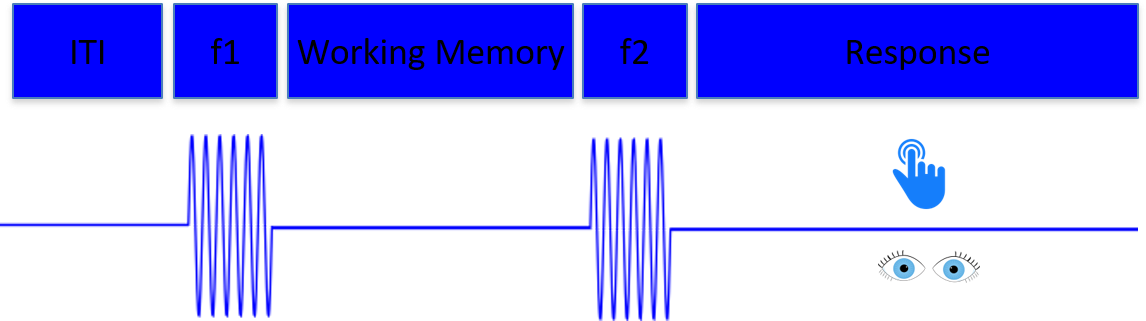
\includegraphics[width=1\textwidth]{figures/SFC_task.png}
\caption{Sequential frequency comparison (SFC) task. Two vibrotactile frequencies are presented to the index finger in succession, $f1$ and $f2$. The task is to decide whether $f2$ is larger than $f1$ or vice-versa. Between $f1$ and $f2$ is a working memory interval in which the frequency of the first stimulus has to be retained. After perception of $f2$, responses are made, typically via button press or saccade.}
\label{fig:SFCtask}
\end{figure}
The task is to decide whether the second ($f2$) frequency is higher or lower than the first ($f1$). To solve this challenge the subject must sequentially go through cognitive processes that are classically split into four parts. First, $f1$ is perceived. Second, $f1$ is being kept in memory, while the subject waits for the subsequent stimulus. Third, $f1$ is compared with the perception of $f2$, thereby forming a decision.  Fourth, the subject reports the choice, usually by pressing a button or enacting a saccade to a choice-specific visual target.
\subsection{Sequential comparison tasks: perception}
Perception of the first stimulus drives quickly adapting (QA) neurons in Brodmann areas 1 and 3b of the contralateral primary somatosensory cortex (SI). These neurons receive afferent signals from mechanoreceptors in the skin, which are routed via the Thalamus and are closely interconnected \parencite{Merzenich1969,Mountcastle1967,Talbot1968}. The majority of monkey SI neurons align their spiking activity to the periodicity of the stimulus, which can also be observed in human M/EEG as steady-state evoked potentials/fields (SSEP/F) \parencite{Mountcastle1990,Nangini2006,Tobimatsu1999}. Moreover, a portion of S1 neurons increase their firing rate monotonically with increasing vibrotactile frequency \parencite{Hernandez2010,Hernandez2000,Lemus2010,Luna2005,Salinas2000}. Notably, only those QA neurons that modulate their firing rates by the vibrotactile frequency showed differential patterns in error trials, indicating that the brain uses these neurons to inform behaviour \parencite{Salinas2000}. Therefore, it is well-established that the firing rates and the rhythmic SSEF/Ps observed with M/EEG represent the encoding of sensory evidence on which later decisions are based. Interestingly, the firing rate predicts the monkeys’ behaviour better than the periodicity of the neural responses and while periodicity is high in SI, it is almost absent in SII, speaking against a communication mechanism through periodic firing as would be predicted from SSEF/Ps \parencite{Hernandez2000,Luna2005,Salinas2000}. An alternative possibility is that QA neurons encode stimuli by the number of discrete bursts of spikes instead of single spikes. Such a coding scheme has been observed in visual tasks and has been suggested to efficiently encode stimulus features  \parencite{Kepecs2003,Kepecs2002,Krahe2004,Reinagel1999,Romo2013}. Notably, because other relevant monkey work has focused on bursts \parencite[e.g.,][]{Lundqvist2016}, the stimulation times extend beyond the time of a burst in these vibrotactile studies (always 500ms) and therefore a code based on spikes is indistinguishable to one based upon bursts \parencite{Romo2013}. However, it remains unclear if bursting covaries with behavioural performance on a trial-by-trial level as has been observed for spikes \parencite{Luna2005}. Regardless whether bursting or spiking underlies an encoding by rate, such a code could be positively or negatively correlated in upstream areas, as is observed throughout the sensorimotor hierarchy in this task including SII, prefrontal and motor cortices \parencite{Hernandez2010,Salinas2000}.

\subsection{Sequential comparison tasks: working memory}
Such a dual rate code, with populations either increasing or decreasing with stimulus frequencies, was also observed in the absence of stimulation: during the short retention interval between $f1$ and $f2$. In particular, \textcite{Romo1999} recorded from the inferior convexity of the prefrontal cortex and identified neurons whose firing rate changed monotonically with the vibrotactile frequency held in working memory (WM). Visual tasks have long associated sustained prefrontal firing with WM \parencite{Funahashi1989,Fuster1971,Goldman-Rakic1995}, however, this study demonstrates that the contents of WM can directly map onto firing rate changes in single neurons. Further analyses indicate that the representation of stimulus information by population dynamics of prefrontal neurons degrades after stimulus presentation, but re-emerges with different tunings towards the end of the working memory delay \parencite{Barak2010}. This is particularly interesting, because it challenges the view that WM is encoded in sustained firing throughout delay periods, with biophysically plausible alternatives both in rhythmicity \parencite{Fiebig2017,Lundqvist2018a,Lundqvist2016} and synaptic changes \parencite{Mongillo2008,Stokes2015}. This current high-level debate \parencite[for either side, see:][]{Constantinidis2018,Lundqvist2018} is so interesting for vibrotactile SFC studies, because firing rates directly represent the contents of WM, not overall changes. Recent evidence, however, suggests that both single neurons and populations may be responsible for WM in this task. \textcite{Haegens2017} recorded local field potentials (LFPs), which reflect local neuronal ensembles, and single neurons from monkey premotor cortex during a multimodal version of the SFC task. They found a modulation of LFP beta oscillations reflecting the stimulus features during WM. In addition, premotor spike-field coherence with the beta band was also related to the stimulus features, indicating a tuning of firing rate to this rhythm. These findings suggest that both population-related beta modulations and the closely affiliated spike activity encode the contents of WM.

This close coupling of beta oscillations with spiking activity underlying tactile WM has also been suspected from a series of EEG studies. \textcite{Spitzer2010} gave human volunteers a similar SFC task and found a parametric modulation of the beta band in the right inferior frontal gyrus (IFG), suggesting that both monkey and human prefrontal cortices (PFC) exhibit content-specific activity during WM. In a follow-up study, \textcite{Spitzer2011} demonstrated that this prefrontal activity was independent of encoding processes, by retro-cueing to one of two presented vibrotactile stimuli. Furthermore, \textcite{Spitzer2012} hypothesized that this parametric encoding of abstract magnitudes was supramodal. In addition to the tactile task, they implemented a sequential visual flicker and a sequential acoustic flutter comparison task. Across all these modalities, prefrontal beta power monotonically encoded the frequency information of the stimulus. However, this parametric code consists of a monotonic increase in beta power with the vibrotactile stimulus held in working memory and did not exhibit the negative component of a dual code as had been observed in monkey PFC \parencite{Romo1999}. Because the precise link between the large-scale signals recorded with EEG and single neuron firing rates are poorly understood, it remains unclear whether the difference in power reflects a population imbalance of the dual code observed in monkeys, where about 60\% of modulated neurons reflected a monotonic increase \parencite{Romo1999,Spitzer2010}. This is of particular note, because working memory has been associated with sustained firing rates in the PFC \parencite{Funahashi1989,Fuster1971,Goldman-Rakic1995,Pasternak2005} and gamma, not beta, appears to be closely related to neural firing rates even when recorded with surface EEG \parencite{Whittingstall2009}. However, increases in gamma activity during working memory do not necessarily reflect sustained firing rates, but a more dynamic system of neural firing patterns \parencite{Cromer2010,Durstewitz2006,Shafi2007,Stokes2013}. Indeed, recent monkey recordings revealed a pattern of brief gamma bursts accompanying encoding and re-activation of stimulus information while beta bursts reflected a default state of maintenance that was interrupted by gamma \parencite{Lundqvist2016}. Notably, it is quite possible that such short gamma bursts have been averaged out of datasets by summation over multiple trials to increase the signal to noise ratio in previous human recordings \parencite{Stokes2016}. Furthermore, during EEG recordings the skull acts as a low-pass filter \parencite{Pfurtscheller1975}, making it difficult to pick up on gamma oscillations. The only MEG study investigating gamma in an SFC task, found overall gamma increases in SI, SII and frontal cortices during working memory, but did not investigate the parametric encoding of stimulus features \parencite{Haegens2010}. Therefore, it remains an open question how the parametric beta band modulations observed by Spitzer and colleagues are associated with dynamic changes in gamma frequencies. 
\subsection{Sequential comparison tasks: decision making}
The next part of the SFC task, comparing $f1$ and $f2$ to form a decision is associated with neural firing in premotor cortices (PMC) that are modulated by subtracting $f1$ from $f2$ \parencite{Hernandez2010,Hernandez2002,Jun2010,Romo2004}, which has also been observed in SII \parencite{Romo2002}. Notably, the decisions were indicated by button press and therefore likely associated with PMC rather than with FEF when responses are indicated with saccades \parencite[see also][]{Gold2007}. Underlining this function, the PMC firing rates were modulated reversely during incorrect trials, indicating that they followed the monkey’s choice rather than the physical attributes of the stimuli \parencite{Hernandez2002,Romo2004}. Most interestingly, because the retention of vibrotactile stimuli was associated with beta power in humans \parencite{Spitzer2010}, \textcite{Haegens2011} recorded local field potentials (LFPs) from monkey PMC and found that beta band power reflected the difference between $f2$ and $f1$. Importantly, when monkeys were instructed to respond independent of the task, neural firing and beta LFPs were not modulated by the decision process in PMC \parencite[see also][]{Haegens2017}. These findings in monkeys correspond well to recent EEG studies extending a role of the beta band for decision making to humans during this task \parencite{Herding2016,Herding2017}. Agreeing with \textcite{Haegens2011}, \textcite{Herding2016} demonstrated that beta band power in premotor areas was modulated by participants’ choices, always with the decision outcome $f2>f1$ resulting in a larger beta response than the outcome $f2<f1$. These same findings were replicated for saccade responses, and in line with an intentional framework for decision making \parencite{Shadlen2008}, the beta modulation was source localized to the FEF instead of PMC \parencite{Herding2017}. Moreover, these studies used Bayesian modelling of participants’ behaviour to estimate the subjective contribution of beta to choices, revealing both a clear pattern of beta invariant to the response mapping (index/middle finger) and a scaling by choice even when trials were incorrect. Yet, it remains unclear whether this choice-related beta band effect in the EEG extends beyond somatosensory processing, which has been associated closely with this frequency band \parencite{Pfurtscheller1981}. 

Building upon this finding of choice-related beta modulation, \textcite{Ludwig2018} added a response delay to this task, in which the response mapping was not provided. With this slight change in setup, they found an almost identical beta band effect in the posterior parietal cortex (PPC), but not in premotor areas. This indicates that premotor areas are only directly involved in the decision process when the decision outcome is known. The PPC on the other hand appears to fulfil an effector-unspecific role and might have a more general role in the decision process. This is particularly interesting, because another parietal signal, the classic P300 \parencite{Chapman1964,Sutton1965}, has long been associated with decision making \parencite{Donchin1967,Rohrbaugh1974}. More so, the P300, recently also termed centro-parietal positivity (CPP - more on it later), has been theorized not to reflect a unitary neural event after stimulus onset, but a dynamically changing neural signature of making a decision over time \parencite{Twomey2015}.  Thus, the question remains how the choice related beta band effect in SFC tasks relates to decision signals in other paradigms, specifically the CPP and beta-gamma modulations observed with MEG in accumulation of evidence tasks \parencite{Donner2009,Donner2007,Kelly2013,Kelly2015,OConnell2012,Twomey2016,Twomey2015,Philiastides2014}
\section{Accumulation of evidence tasks}
The other line of research I want to introduce builds also on Fechner’s work on psychophysics, and in particular is the result of his legacy in mathematical psychology that drove ever-improving accounts of choice behaviour throughout the 20th century. This led to the development of signal detection theory, which as previously mentioned, has the advantage of taking into account noise behaviour and the structure of incorrect trials \parencite{Tanner1954}. Neuroscientific experiments have used this theory to model perceptual decision making as a process of sequential sampling that results in an accumulation of evidence for a decision. Underlying this model is the idea that a decision variable (DV) represents the set of all evidence for a decision and for binary choices modern models posit a single mechanism that accumulates evidence over time for one choice over another \parencite{Shadlen2013}. For example, in our introductory example when we strive to find a good watermelon stand, we would sample melons from one stand sequentially, until we are sure the stand sells fruit of high or low quality. Every time we try a fruit, we would get a piece of evidence in favour of one possible choice, which over time accumulates to inform a decision – typically modelled as crossing an absolute bound. The neuroscientific hypothesis is that one decision variable tracks the current state of such evidence accumulation and that we can observe such a variable in the brain. 

To track this neural correlate of perceptual decision making, neuroscientists have used predominantly one decision making task: the random-dot motion (RDM) direction discrimination. In the RDM task (figure \ref{fig:RDMtask}) participants are shown dots on a monitor that move around. A portion of these dots move coherently in the same direction and the challenge is to detect this movement. Because the number of dots moving coherently is typically low and movement can only be spotted through a change over time, the perceptual challenge is usually difficult, and it can take between a few hundred milliseconds to seconds to detect the motion. Moreover, because the dots typically move randomly, it is possible to perceive a wrong direction.

\begin{figure}[t]
\centering
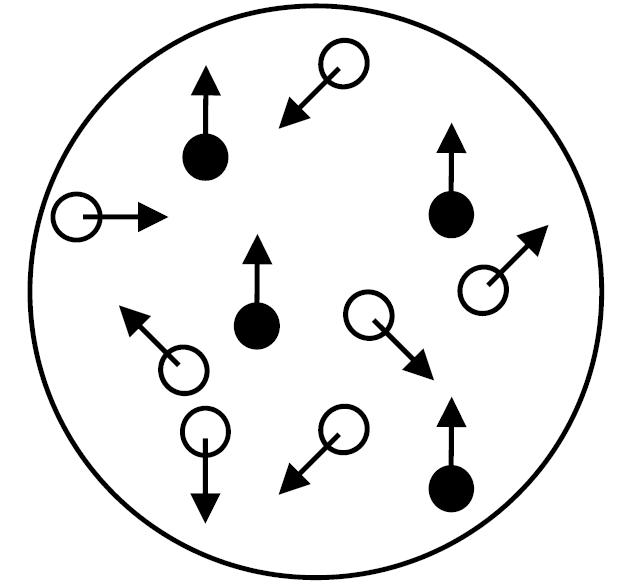
\includegraphics[width=.3\textwidth]{figures/RDM_task.png}
\caption{Example of random-dot motion kinematogram. The white dots represent the dots moving randomly, the black ones the coherently moving dots. The task is usually to detect coherent motion, varying the number of coherently moving dots determines the difficulty and time needed to perform the judgement.}
\label{fig:RDMtask}
\end{figure}

This task is particularly powerful for psychophysics, because it requires no distinct working memory process and it lends itself well to be modelled as an accumulation-to-bound process \parencite{OConnell2018}. In such models it is assumed that subjects continuously sample from the dot-motion stimulus, perceive the motion direction of individual dots and accumulate evidence for one direction over time. When participants have a level of confidence in the direction, the decision bound is crossed and the decision communicated. This is usually done in monkey experiments by eye movements. The model can be further simplified by having the subjects decide between two opposite directions that are known in advance, thus becoming a binary accumulation process. Notably, because choices are typically indicated by performing a saccade to one of two targets associated with the choices, the decision process can be treated as a process of movement selection. Therefore, beyond motion sensitive neurons in MT/V5, recordings are primarily carried out in those areas associated with motor preparation and eye-movement execution, resulting in neural correlates of a decision variable in the superior colliculus (SC), frontal eye fields (FEF), lateral intraparietal area (LIP) and the dorsolateral prefrontal cortex (DLPFC) \parencite[for review see][]{Gold2007}. 

\subsection{Accumulation of evidence tasks with nonhuman primates}
Employing the RDM task while recording from macaques, \textcite{Britten1992} were able to link a small set of middle temporal visual area (MT/V5) neurons to concurrent choice behaviour. Even when the coherence was at 0\% and all dots were moving randomly, MT firing rates predicted choices significantly \parencite{Britten1996}. Motion sensitive neurons in area MT are well-known to respond strongly to visual stimuli moving in a particular direction, exhibiting tuning to stimuli moving through their receptive fields \parencite{Baker1981,VanEssen1981,Zeki1980,Zeki1974}. Using this knowledge of systematic motion direction organization in MT, microstimulation has been used to successively activate motion direction specific systems, thereby demonstrating a causal relationship of MT neurons for task performance \parencite{Ditterich2003,Salzman1990,Salzman1992}. Most interestingly, when using a version of the RDM task with the opportunity to respond as soon as possible, MT microstimulation influences both choice and RTs in the stimulated neurons’ preferred motion direction. In turn, when MT neurons are deactivated, the decision making process is impaired, likely because the sensory encoding is interrupted \parencite{Katz2016}. On a functional level these findings indicate that MT processes the motion information and thus provides the sensory evidence on which decisions are formed.

To find out the neural substrates of a decision variable, a large body of monkey recordings targeted the FEF, because it is well-connected to visual areas, and known to encode the saccade processing required to respond in the RDM paradigm \parencite{Felleman1991,Hanes1996,Schall1995,Schall1995a,Thompson1996,VanEssen1992}. Moreover, suprathreshold electrical stimulation evokes saccades while subthreshold stimulation elicits changes to saccade selection and spatial attention \parencite{Burman1997,Moore2001,Moore2003,Robinson1969}. \textcite{Gold2000} interrupted motion viewing during the evidence accumulation process while monkeys viewed the RDM stimuli. Then they immediately applied a short electrical current to the FEF, which resulted in a saccade whose direction and amplitude was influenced by the current state of the decision process, reflecting the evolution of a decision variable \parencite{Gold2000,Gold2003}. However, while the FEF is clearly involved in the decision process, it appears that only a small part of FEF neurons track the DV, while others encode stimulus properties during and after the decision, possibly to evaluate the outcome \parencite{Ding2012}. Together, these studies indicate that the FEF is related to action-performance in RDM tasks with saccade responses, but also encodes stimulus and outcome related information.

Besides the more perceptual aspects of MT and the action-related activity in FEF, the lateral intraparietal area (LIP) has been extensively studied in RT-dependent versions of the RDM task. LIP has been focused on, because anatomically it receives inputs from MT and outputs to the FEF \parencite{Andersen1992,Blatt1990,Lewis2000}. In particular, the LIP is tightly coupled to areas involved in eye movement control \parencite{Andersen1990}. LIP neurons fire when a saccade is planned into their receptive fields \parencite{Andersen1987} and its neurons fire persistently when an animal withholds a saccade to a target \parencite{Barash1991,Gnadt1988}. Thus, LIP function appeared to be between perceptual processing and eye-movement execution, responsible for sensorimotor integration mediated by cognitive control \parencite[for review,][]{Andersen2002}. Therefore, it was unsurprising when \textcite{Shadlen1996,Shadlen2001} demonstrated that activity in LIP neurons, whose receptive fields were aligned with visual targets in the RDM task, increased before saccades to these targets were executed. Surprisingly however, single neuron activity was modulated by the presentation of dot-motion and correlated with RDM coherency. That is, activity reflected the difficulty of individual RDM patches by faster increases of firing rates in easy trials, indicating that LIP neurons tracked the evolution of the decision process. Most interestingly, LIP firing rates accumulated to a fixed threshold at the time of response independent of trial difficulty, fitting to drift-diffusion models of decision processing \parencite{Roitman2002a,Shadlen1996,Shadlen2001}. Contrary to MT however, LIP microstimulation appears to only slightly affect choice and RT \parencite{Hanks2006}. Moreover, when short motion pertubations were added to the RDM kinematogram, RT and choices were modulated by these over a sustained period of time \parencite{Huk2005}. Together, these findings indicate that LIP neurons reflect the integration of decision information over time and microstimulaton pertubations drive the encoded decision variable with respect to a decision bound. 

Most relevant to the present thesis (task design study 1 \& 3), when responses could not be immediately taken and monkeys had to map targets to a spatially undetermined color-code, LIP neurons still represented the DV even though no specific saccade planning was possible \parencite{Bennur2011}. This indicates that LIP function includes tracking the evolving DV independent of a specific motor response. However, a recent study using causal de-activation of LIP neurons during decision formation suggests that LIP neurons may not be critical for computing perceptual decisions, and may only reflect secondary processes that correlate with the actual computation \parencite{Katz2016}. This is particularly interesting, because concurrent recordings from six regions involved in decision making including MT, FEF and LIP suggest that information is not confined to specific cortical regions but shared among relevant brain areas and transmitted via bursts \parencite{Siegel2015}. This observation ties in well with earlier studies suggesting that decision information is present even in areas functionally specific to early visual processing and may be communicated there via feedback from downstream cortices \parencite{Donner2008,Nienborg2009,Siegel2011}. If information is shared along the whole perception-action loop in a network between distributed regions, studying the whole system instead of isolated areas might be necessary, as is done in human neuroimaging. 

\subsection{Accumulation of evidence tasks using M/EEG in humans}
Studies of perceptual decision making with nonhuman primates have discovered that many different areas throughout the cortical hierarchy are involved and share information across large distances. Yet, we know little about how these areas dynamically interact to form decisions, because studies recording from single cells are always limited to small populations and few cortical areas. In contrast, studies using neuroimaging with human subjects can trace neuronal dynamics across the whole head and concurrently throughout cortices. In addition, human subjects can be asked directly on what their perceptions and decisions were, e.g. how confidently they made a choice, and are recorded in much larger number, leading to better inferences about common mechanisms. Notably however, little is known about how many of the rhythms measured with M/EEG correspond to single-cell recordings and how they compare to signals detected in fMRI BOLD contrasts \parencite{Buzsaki2012,Jann2010,Keller2013,Lee2014,Logothetis2001,Scheeringa2011,Whittingstall2009}. 

Coherent oscillations between cortical areas may dynamically regulate the information flow across sets of neuronal populations \parencite{Engel2001,Fries2015,Salinas2001,Sejnowski2006,Varela2001} and MEG is well-suited to study such cortical dynamics \parencite{Siegel2011}. Using MEG to discover the role of cortical oscillations for perceptual decision making, \textcite{Donner2007} asked human volunteers to detect RDM motion (rather than choosing between directions) and found that beta power was elevated throughout the dorsal visual pathway including MT, intraparietal sulcus (IPS) and dlPFC for correct vs. incorrect trials. Interestingly, this activity predicted the accuracy and not the content of the upcoming choice, suggesting that beta reflected the computation of decisions rather than the content \parencite[see also][]{Siegel2011}. In another experiment, volunteers were shown an RDM patch at different coherence levels and had to indicate the motion direction \parencite{Siegel2007}. After a typical event-related field, they observed a parametric scaling of occipital gamma power with the stimulus coherence and the opposite, but less robust, pattern in alpha and beta bands. Because the visual areas partial to this effect are known to be involved in motion processing, such as MT, this suggests that gamma reflects processing of the evidence on which decisions are based. 

To investigate the action component of such perceptual choices, in another experiment \textcite{Donner2009} presented RDM stimuli for a fixed time and before responses were given with either hand, a short delay was enforced onto the participants. Gamma band activity increased over the contralateral (pre-) motor cortex, and low frequency alpha and beta oscillations decreased with respect to the ipsilateral hemisphere. Notably, this pattern built up during stimulus viewing, likely reflecting the accumulation of evidence for a decision that would be source localized to FEF when responding with saccades instead \parencite{Herding2017}. The lateralization of beta-band activity over central electrodes in particular appears to reflect an emerging motor plan that is directly associated with participants’ choices. Building upon this finding, \textcite{DeLange2013} demonstrated that pre-stimulus variance of lateralized power in the beta band predicted choices and that the accumulation of beta lateralization was modulated by motion coherence. In sum, these MEG studies demonstrate signals corresponding to the sensory processing in MT and the action-related activity in FEF as observed in nonhuman primates and suggest an active role of beta and gamma oscillations in encoding the stimulus content. However, monkey studies have found extensive correlates of neuronal activity in the posterior parietal cortex with the evolution of a decision variable, which could not be identified with MEG. This is particularly curious, because recent EEG studies have observed consistent evidence of a centro-parietal potential (CPP or P300) that may be a candidate signal for such a parietal mechanism \parencite{Kelly2015}.  

The CPP has been identified as a rhythm matching the evolution of a decision variable during perceptual decision making tasks \parencite{Kelly2013,Kelly2015,Philiastides2014,Twomey2015}. One strategy to find this signal in RDM tasks has been to eliminate the typically observed ERPs resulting from stimulus onsets by presenting a field of randomly moving dots before coherent motion onset, thereby allowing for a seamless transition \parencite{Kelly2013}. Moreover, responses are often made by button press using either left or right hands, to enable observation of lateralized beta power \parencite[as in][]{DeLange2013,Donner2009}. Using this setup, \textcite{Kelly2013} recorded EEG while humans performed the RDM task. They found that the CPP exhibited an accumulation-to-bound with respect to the decision of up- vs downward motion. In addition, the rate of CPP build-up was modulated by the sensory evidence strength, exhibiting a defining property of theoretical accounts of a decision variable. Even though effector specific activity in form of the lateralized readiness potential \parencite{Eimer1998,Smulders2012} did also show a ramping up, this activity was driven by the abstract, centroparietal signal. Moreover, in a previous study with a change detection task, hand movement specific motor signals, such as the previously observed beta lateralization, also exhibited a pattern of build-up to a threshold just before responses were executed, however, were abolished when manual responses were not carried out \parencite{OConnell2012}. This indicates that the CPP appears one directional in this process and only represents the accumulation-to-bound in a positive manner. This means that it doesn’t represent different choices – a signed value - but the absolute value of the DV. The effector-specific beta activity on the other hand includes information about choices, because they have to be enacted on. Such an interpretation of the CPP  is in line with observations in LIP neurons and theoretical accounts that posit the supramodal accumulation of evidence for distinct alternatives in the same cortical areas that race each other \parencite{Brown2008,Roitman2002,Usher2001}. Moreover, recent evidence suggests that neural correlates of a DV are independent of motor plans in LIP \parencite{Bennur2011} and corresponding human area IPS includes distinct systems implementing motor and perceptual decisions, suggesting functional heterogeneity \parencite{Filimon2013}. Therefore, it remains unclear what exactly is encoded by the centroparietal signals observed with EEG from this area and what precise cognitive function underlies the ramping up of activity.

If the CPP is the same signal as the P300, as recently suggested  \parencite{Twomey2015}, then a large body of evidence has indicated a relationship with a plethora of alternative cognitive processes \parencite{Nieuwenhuis2011,Nieuwenhuis2005}. One measure in particular appears to fit well to recent observations of the CPP: confidence \parencite{Hillyard1971,Squires1973}. Because the CPP is not selective in its accumulation for one choice over another, it may only reflect the absolute value of a DV. Such a signal is closely related to confidence, which can be viewed as the distance between the DV and the closest decision bound \parencite{Urai2014}. A confidence signal would therefore not be selective for choices; however, it would still be affected by them. If participants commit an error, the DV should reach the same threshold as in a correct trial, while confidence should be lower \parencite{Shadlen2013}. Most interestingly, \textcite{Philiastides2014} used a face-house discrimination task in which participants also had to sequentially sample and integrate information over time. They found that a CPP gradually built-up over time with the amount of evidence for either choice, as predicted from drift-diffusion models (DDM) and corresponding to RDM tasks. However, the signal did not reach a fixed threshold, but was still modulated by the amount of evidence for a choice. Because a simple DDM could not account for this, the authors demonstrated that adding a proxy for confidence on each trial could. This indicates that at the time of response, the CPP includes information about choice confidence. However, participants weren’t specifically asked how confident they were in their decisions, and it remains unclear whether this part of the CPP can be related directly to confidence judgements, as has been done in fMRI \parencite[e.g.,][]{Hebart2016}.

\subsection{Accumulation of evidence tasks using fMRI in humans}
Functional magnetic resonance imaging (fMRI) has indeed provided another avenue of human neuroimaging research to investigate perceptual decision making and confidence with high spatial acuity. \textcite{Heekeren2004} gave participants a similar face-house discrimination task as described in the previous section \parencite{Philiastides2014} and used the spatial specificity of face processing in the fusiform face area (FFA) and house processing in the parahippocampal place area (PPA) to investigate relative blood-oxygen-level dependent (BOLD) increases. BOLD is known to increase in the FFA and PPA when faces and houses are perceived, respectively and can be related to single neuronal codes for either stimulus \parencite{Epstein1998,Haxby2000,Ishai1999,Kanwisher1997,Logothetis2001,Logothetis2004,McCarthy1997}. A region responsible for decision making should covary with either FFA or PPA activity depending on whether faces or houses were perceived \parencite{Heekeren2004}. Because the BOLD response is sluggish, it can only pick up on the overall activity during a trial and a modulation by evidence in either area is likely difficult to detect. However, the authors postulated that a candidate decision making area should show a pattern of easy trials associated with higher BOLD responses than hard trials, because in easy trials BOLD responses should reach a high level faster. They found that the left dorsolateral PFC (dlPFC) showed such an activity pattern and in a follow-up demonstrated that this was independent of the response modality \parencite{Heekeren2006}. In addition, the role of the dlPFC appears to be one of integrating evidence, modeled as the drift in DDM, because when repetitive transcranial magnetic stimulation (TMS) was applied to this area to interrupt the decision process, accuracy and response times were stymied in line with an interpretation as decreasing drift rate \parencite{Philiastides2011}. Notably in the context of the present thesis, this prefrontal activity appears to be co-activated with the IPS and FEF, suggesting a frontoparietal network involved in encoding of stimulus information and decision making \parencite{Heekeren2006,Ho2009,Kayser2010,Liu2011}. In particular, \textcite{Liu2011} designed an RDM task where they gave information about the response modality, either button press or saccade, before or after the stimulus presentation (\href{https://doi.org/10.3389/fnhum.2017.00576}{see design of study 1 of this thesis}). Because participants could answer as fast as they wanted, with no forced delay as in \textcite{Heekeren2004}, the BOLD responses were increased for more difficult trials \parencite{Hanks2017}, indicating that participants accumulated evidence for a longer time. Besides frontal areas and the anterior insula, the modulation was present in saccade-related areas FEF and IPS. Crucially, the foreknowledge and response modality did not have an effect on this activity pattern, suggesting no effector specificity of the neural system underlying evidence accumulation. These findings fit well with recent observations in monkey LIP, indicating that information about RDM direction was present before monkeys knew where the saccade target was going to be \parencite{Bennur2011}. 

Together, human neuroimaging provides a complimentary view to monkey recordings and provides evidence for the involvement of prefrontal and parietal areas in perceptual decision making\footnote{In addition, fMRI has revealed a role for the anterior insula during evidence accumulation \footcite{Ho2009,Liu2011}. Because the insula is related to many different cognitive functions and because the present studies haven’t found signals corresponding to such activity, I have left this introduction for another place \footcite{Menon2010}.}. Most notably, the dlPFC appears to fulfil the role of a domain general evidence accumulator, not evident from monkey single-cell recordings. Apart from these prefrontal findings, human fMRI and M/EEG studies show a remarkable similarity with monkey recordings in the areas involved in perceptual decision making. Especially the pattern of parietal signals tracking the evidence accumulation of noisy input and (pre-) motor areas exhibiting variability with the execution of choices is consistent across species and methods. Moreover, it appears that the information about the current state of decision making, a DV, is available to many areas and not restricted to a central decision maker. This is particularly important, as neural oscillations studied with M/EEG often reflect the dynamics of a cortical representation. More so, the dynamics of a general decision making mechanism are likely to be similar across cognitive tasks, such as the RDM and the SFC task, even if sensory modality or stimuli involve distinct cortical areas.

\subsection{Common neural codes across perceptual decision making tasks}

Evidence of common neural codes was found in studies using the RDM stimulus in a sequential comparison setup. \textcite{Zaksas2006} recorded from areas MT and PFC, while monkeys performed a delayed match-to-sample task on the motion direction of two sequentially presented RDM stimuli. During perception of the first stimulus, MT and PFC neurons were direction selective, but selectivity in PFC emerged 40ms after MT. During the delay period, neurons in both areas were attuned to direction, but through transient, not sustained firing. Similarly, the decision information was present in both MT and PFC, but the PFC was modulated 100 ms later and predictive of the upcoming choice. This indicates that PFC neurons encode task-relevant features about visual motion and represent the decisions that are based on comparisons taking place in MT. In addition, \textcite{Hussar2012} recorded from two distinct principal types of PFC neurons, pyramidal and interneurons, during the same task. They found that while both were involved in perception, mostly pyramidal cells carried information throughout the delay period, in a transient, dynamic code. Furthermore, the cell type determined whether the neuron was attuned to matching versus non-matching RDM directions. This suggests that the PFC employs a dual code for decision making in which different cell types have distinct contributions. To investigate the network states involved in this visual comparison task, \textcite{Wimmer2016} analysed LFPs from the lateral PFC from monkeys comparing either the motion directions or speeds of two RDM patches. During perception, theta and gamma power was increased, while beta decreased. In the subsequent delay, beta power encoded the relevant RDM feature, agreeing with findings in human neuroimaging \parencite{Spitzer2010,Spitzer2012}. Broadband LFP activity reflected the difference between S2 and S1 and was split into an early signed modulation (S2-S1) and a later absolute choice-related component that reflected the buildup of the perceptual decision. Albeit in different areas, these results appear remarkably similar to findings of decision beta in SFC tasks on the one hand \parencite{Haegens2011,Herding2016}, and the CPP \parencite{Kelly2013} on the other. However, until the studies included in the present thesis, there have not been any human neuroimaging approaches investigating these common cortical dynamics. 

\section{Objectives of this dissertation}

Throughout the research for this dissertation, my primary aim has been to find the neural substrates underlying working memory and decision making with the intention to understand these cognitive functions better. Neural oscillations have been associated with these specific mental tasks, however, several important questions on the role of beta and gamma oscillations, in particular, remain unanswered. I addressed these gaps in our knowledge in three studies using a sequential comparison task with tactile (study 1+2) and visual stimuli (study 3). Moreover, I bridged the gap of perceptual decision making research using the predominant random-dot motion stimuli in a new comparison task setup (study 3). In conjunction with neural oscillations, I investigated broadband centro-parietal signals, and related them to motor beta, trial difficulty and confidence (study 2+3). Finally, this thesis accumulates the information from these three very related studies and outlines common themes surrounding the beta and gamma band as well as possible common ground with the CPP. 
\cleardoublepage
% !TEX root = ../Dissertation-vonLautz.tex

\chapter{Summary of original research articles}

%%%%%%%%%%%%%%%%%%%%%%%%%%%%%%%%%%%%%%%%%%%%%%%%%%

\section{Study 1: Gamma and Beta Oscillations in Human MEG Encode the Contents of Vibrotactile Working Memory}
From single-cell recordings in monkeys to large-scale human EEG, the parametric encoding of vibrotactile frequency during working memory is well-established \parencite{Romo1999,Spitzer2010}. As reviewed in the introduction, a number of recent EEG studies have identified cortical oscillations in the beta band to represent the frequency information during a short delay in a vibrotactile sequential frequency comparison task. However, visual and auditory working memory studies have found a crucial role of gamma oscillations for working memory, not observed in previous vibrotactile EEG studies \parencite{Roux2014}. In addition, the only MEG study investigating tactile working memory found a modulation of SI and - most interestingly - of SII during stimulus retention, but didn’t investigate a parametric modulation in prefrontal areas \parencite{Haegens2010}. While the authors did find an overall increase in frontal gamma during WM, this was limited to contrasting periods of working memory with a prestimulus baseline and was not content specific. Therefore, our first goal was to investigate whether frontal gamma was encoding stimulus features during WM. In addition to this aim, a line of monkey and human neuroimaging studies has identified the intraparietal sulcus (IPS) as a hub for numerosity processing, a mental task very similar to the vibrotactile features in our design \parencite{Nieder2016}. However, studies using EEG have not been able to localize IPS activity reflecting the vibrotactile frequency held in WM as is known from fMRI \parencite{Wu2018}. Therefore, we aimed at detecting both high frequency oscillations in the gamma band and stimulus information from the IPS for the first time.

We recorded 306-channel whole-head magnetoencephalography while participants performed a version of the vibrotactile frequency comparison task. Notably, our original task design intended to also investigate how beta-gamma codes of decision making were influenced by foreknowledge of the response modality, and therefore the task included responses with button press and saccades. However, due to technical problems, we had to discard the analysis of decision making related activity. 

Our main analysis probed with a zero-mean contrast of the four different vibrotactile frequencies held in working memory at 15, 19, 23 and 27 Hz, whether there were channels, frequencies or time points in which a parametric code of vibrotactile frequencies was present. With a nonparametric cluster-based permutation test we identified three areas that showed such a pattern, all around the center of the WM interval. First, replicating previous EEG findings, beta power in the right IFG at around 30-35 Hz. Second, low beta power (10-20Hz) in bilateral parietal channels which was source localized to the IPS. Third, matching the beta effect in source location in the right IFG, gamma power (74-90 Hz) was negatively modulated by the vibrotactile frequency, thus showing the opposite pattern of the beta band effects. Notably, we did not replicate effects of overall broadband gamma power increases in SI, SII and frontal cortices as had been observed in a similar vibrotactile task \parencite{Haegens2010}, while replicating essentially all other patterns typically observed in vibrotactile SFC tasks with M/EEG \parencite{Bauer2006,Spitzer2010}. 

These results indicate that there is a frontoparietal network underlying the retention of vibrotactile stimuli with an extended role of the beta band that may interact with gamma to enable working memory. We demonstrate for the first time with MEG that the IPS is also involved in this process and that the gamma band, which is associated more directly with neuronal firing than beta, might drive the prefrontal processing \parencite{Lundqvist2016,Whittingstall2009}. Future MEG studies should investigate the network configurations of such processes, through analyses of cross-frequency coupling in a longer working memory period or the extraction of frequency-specific time courses with high temporal resolution \parencite{Vidaurre2016,Vidaurre2018}.

\section{Study 2: Neuronal Signatures of a Random-Dot Motion Comparison Task}
Both the vibrotactile frequency comparison task and the random-dot motion task have been studied extensively in humans and monkeys as I introduced earlier. However, there is remarkably little research aiming at finding common codes across these perceptual decision making tasks. So far, no human neuroimaging study has investigated the RDM task with vibrotactile stimuli nor studied the sequential comparison of random-dot motion stimuli. This is particularly curious, because pupillometry in humans and electrophysiological recordings in monkeys using a combination of these classical tasks have produced high-impact studies that give novel insights into the encoding of decision information \parencite{Urai2017,Wimmer2016}. Here, we recorded EEG while human volunteers were tasked to compare the coherence of two sequentially presented random-dot motion stimuli ($S1$, $S2$) and responded by button press. If findings from SFC studies indeed transfer to the visual domain, we should observe a parametric beta band code in PFC as well as a modulation of premotor beta by choice. Moreover, RDM stimuli should elicit typical visual effects as well as a correlate of the accumulation of evidence. Crucially, the decision variable in this task reflects the comparison of the first with the second stimulus, thus we should not observe a CPP during perception of $S1$. Moreover, the CPP should scale with the difference between the two, not the coherence of $S2$.

We asked 28 subjects to perform this task and used their behavioral data to model the subjectively perceived coherence difference (SPCD) for each subject and trial. Using variational Bayes, our model accounted for the time-order effect/error \parencite{Hellstrom1985}, a bias typically observed in sequential comparisons. In analogy to study 1, our WM analysis was a parametric contrast of the four $S1$ coherence levels. To look into the decision making interval, we performed a $2x2$ GLM of choice ($S2>S1$ vs $S2<S1$) and performance (correct vs incorrect). Moreover, we investigated the CPP and contrasted it by subjects’ choices and each trial’s SPCD in three levels of ‘easy’, ‘medium’ and ‘hard’.

In our WM analysis we found a significant cluster of prefrontal channels that were modulated by the level of $S1$ coherence retained throughout the inter-stimulus-interval. In agreement with previous EEG studies \parencite{Spitzer2010,Spitzer2012}, this effect source localized to the right IFG, suggesting that the working memory related beta is supramodal and can be observed with stimuli not relying on frequency magnitudes. We also found a negative modulation of gamma, replicating findings from study 1. However, this effect was mainly driven by the lowest coherence stimuli and will require further investigation. Curiously, we also found a negative modulation of low beta band activity by the $S1$ coherence level in centroparietal channels, source localizing to bilateral MI and precuneus.

The analysis of decision-related activity found a modulation of premotor beta band activity 700ms before responses were made that was elevated for choices of $S2>S1$ in comparison to those of $S2<S1$. This is in agreement with recent vibrotactile SFC studies in humans, corresponding in time, frequency and location \parencite{Herding2016} and also agrees with monkey LFPs \parencite{Haegens2011,Haegens2017}. When splitting trials into 3 levels of easy, medium and hard by SPCD, this effect was unaffected, thus reflecting the choices in a binary code. 
The CPP was modulated both in response to the perception of $S2$ and with respect to responses. $S2$-locked activity accrued during the stimulus presentation and stayed on a fixed level afterwards. Crucially, the amplitude of this level was modulated by the trials’ difficulty ($S2-S1’$) and not by the coherence of $S2$. Furthermore, the $S2$-locked CPP was modulated by choice and reached a higher amplitude for choices $S2<S1$ than $S2>S1$, the opposite of the beta band effect. Response-locked CPP showed a pattern of signal accumulation to a peak at the time of response. Notably, this peak was both influenced by choice and the difficulty of trials. At the time of response the CPP did not reach a fixed threshold, like in simple boundary-crossing models, but was scaled by the SPCD, with difficult trials exhibiting smaller amplitudes and incorrect trials demonstrating even smaller amplitudes. This effect was only evident in the last 300ms before responding and in particular, seemed to be driven by a lower starting point to the accumulation rather than variance during the accumulation.

Our findings indicate an extended role of the beta band for both working memory and decision making in comparison tasks, regardless of sensory modality. Beta has been suggested to reflect the “status quo” of information \parencite{Engel2010}. In our studies however, it appears to reflect more than that. It is modulated by the abstract magnitudes in comparison tasks (vibrotactile frequency or RDM coherence) and therefore reflects the WM content, as well as the content of decision making, already very early, 700ms before responding. In conjunction with fast, transient gamma it might therefore reflect the re-activation of content \parencite{Spitzer2017} and/or the maintenance state (also of choice) that is interrupted by gamma \parencite{Lundqvist2018}.

The CPP was strongly modulated by trial difficulty at the time of response, suggesting it reflects a cognitive process that is not wholly explained by crossing a bound in a simple drift-diffusion model. More complex models based on sequential Bayesian updating or with collapsing bounds may be necessary to keep the drift-diffusion view in place. Moreover, it is possible that the CPP reflects an accumulation to an absolute bound, but the signal we observed included other parietal signals encoding the decision confidence. Finally, the CPP was also modulated by participants' choices, indicating a relationship with premotor beta that is yet to be investigated.

In sum, this study was able to bridge gap of decision making paradigms and sensory domains, indicating a common role for beta band driven content encoding and the CPP as an evidence accumulation mechanism that has ties to confidence.

\section{Study 3: Centro-parietal EEG potentials index subjective evidence and difficulty}
The previous study had identified a role for the CPP during sequential comparison tasks, tracking the integration of noisy sensory input over time. It remains unclear however, whether the comparison of two short vibrotactile frequencies elicits a similar response, as this percept does not include the accumulation of noisy evidence over an extended period. Moreover, it remains unknown whether the premotor beta band that scales with subjects’ upcoming choices is related to the CPP. This is particularly interesting, because the CPP reflects the absolute, unsigned strength of accumulated evidence ($|S2-S1|$), while choice dependent beta is a signed value ($S2-S1$) reflecting the direction of the decision. 

In this study, we used EEG data from six variants of the SFC task (n=116) and applied the model based on Bayesian inference to the behavioural data to estimate the subjectively perceived frequency differences (SPFDs). We found that parietal ERPs reflected the SPFCs shortly after the second stimulus offset (168-709ms) in a signed fashion, thus indicating the direction of choice. Crucially, this early parietal signal was correlated with choice-related beta power on a single trial level. While not implying causation, this might be first evidence for a previously unknown EEG signature that indexes the updating of subjective evidence in relation to the ensuing choice. The timing of these two signals as well as their source locations in parietal and premotor cortex further underline the possibility that the early ERPs serve to communicate the evidence for one motor plan or its alternative and the premotor beta band reflects the choice planning based upon this evidence.

In addition to this early parietal modulation by signed difference, we observed later parietal ERPs (273-953ms after stimulus offset) that correlated with the absolute strength of evidence. Interestingly, this later modulation was source localized not only to parietal areas, but also included the bilateral inferior frontal gyrus, which relates it to the parametric encoding of the vibrotactile frequencies during WM. Similar to study 2 we also did not observe an absolute threshold of CPP accumulation, but rather a scaling of the late ERPs by subjective task difficulty. Further analysis revealed that this effect complied to the definition of statistical decision confidence in all aspects \parencite{Hangya2016,Sanders2016}. 

In sum, these findings indicate that early centroparietal ERPs reflect the evidence on which decisions are based, while later modulations might refer to the strength of evidence informing a decision, which is closely related to measures of confidence.
\cleardoublepage
% !TEX root = ../Dissertation-vonLautz.tex

\chapter{General Discussion}

%%%%%%%%%%%%%%%%%%%%%%%%%%%%%%%%%%%%%%%%%%%%%%%%%%
In the research summarized in the previous section, we gained new insights into the role of neural oscillations ascribed to cognitive functions, especially working memory modulated beta and gamma, decision-related beta power and the supramodal nature of the CPP for tracking decisions.

In the first study, we were able to uncover previously hypothesized but never demonstrated modulations of prefrontal gamma and parietal beta power by vibrotactile frequencies held in working memory. Most interestingly, the parietal beta modulations could be source localized to the IPS, an area known to be involved in numerosity processing. These results indicate that a frontoparietal network underlies working memory that employs beta and gamma oscillations in a mechanistic fashion.

The second study encompassed six EEG experiments, whose analysis consistently showed a CPP that accumulated during decision making. With respect to the second stimulus, we observed a scaling of the CPP, first by the subsequent choice and later by trial difficulty, which we relate to confidence. In addition, we found a correlation between choice-related beta and the CPP, suggesting common codes during decision processing. Our findings point to a role of the CPP that goes beyond signaling the status of a DV and insinuate that such a role is related to the decision outcome.

In the most recent experiment, we showed that the functional roles attributed to beta oscillations in the tactile task hold up in a visual variant, indicating a general, supramodal mechanism. Similarly, we demonstrated that non-lateralized choice-dependent beta can also account for decisions when using RDM stimuli. In addition, both stimulus- and response-locked CPPs reflected the tracking of a decision variable during a comparison task that was informed by working memory. This is of particular note, because there was no relationship of the CPP during RDM perception, suggesting independence from sensory processes. Finally, the CPP scaled with subjectively perceived difficulty at the time of response, which further indicates that the CPP incorporates confidence signals.

\section{Unifying accounts of prefrontal beta band oscillations during working memory}

All experiments reviewed here replicated the finding that beta band power from IFG is parametrically modulated by abstract quantitative information (vibrotactile frequency or RDM coherence) held in working memory during a short interval between two stimuli. \textcite{Spitzer2010} had identified this effect at 20-25 Hz with EEG during a similar vibrotactile SFC task. Interestingly, when we used a visual variant of the task, but the same EEG equipment as these authors, the effect was surprisingly similar at 18-26 Hz, however, was found significantly higher (30-35 Hz) in MEG recordings on almost the same vibrotactile task. Because in EEG the skull acts as a low-pass filter \parencite{Pfurtscheller1975} and the observed effect may be an epiphenomenon of averaging further temporally smeared beta bursts, it is quite possible that the prefrontal oscillations even extend into the gamma range. Recent monkey recordings appear to concur with a representation in higher beta oscillations, with a medial premotor beta peak above 25 Hz \parencite{Haegens2017}. This may particularly important, as lower beta modulations (13-20 Hz) occur jointly with alpha \parencite{Hanslmayr2009} and decrease in task-relevant areas while higher beta-band rhythms (20-35) mirror gamma and increase with engagement \parencite{Tallon-Baudry1998}. It may therefore be necessary, in the future, to separate lower beta activity more clearly from higher beta oscillations to avoid grouping them in one beta band.

Our findings in the prefrontal cortex were clearly in the upper beta band and appeared to be related to active processing rather than inhibitory in nature. Enhanced beta has been hypothesized to signal the “status quo” of maintaining the current sensorimotor or cognitive state \parencite{Engel2010}. However, our findings go beyond overall changes. We provide evidence that beta oscillations hold information about the content (vibrotactile frequency or RDM coherence) of working memory on a given trial, joining a growing body of evidence for such a role \parencite{Spitzer2010,Spitzer2011,Wimmer2016}. This type of feature specific activity has also been found in neuronal spiking and high frequency LFPs \parencite{Pesaran2002,Romo1999,Nieder2003} and has been studied extensively with fMRI \parencite{Christophel2012,Christophel2017,Uluc2018,Wu2018}. Yet, it remains unclear how neural activity measured as spike firing rates and BOLD signals relate to the previously observed EEG beta band oscillations. In particular,  it is unknown, whether beta activity correlates positively or negatively with these activity measurements \parencite{Spitzer2017}. Upper beta band oscillations are likely to correspond closer to those in gamma, who have been associated with higher spike rates and increases in BOLD, while low beta may be associated negatively with activity, corresponding to alpha \parencite{Michels2010,Hanslmayr2011}. However, it is also possible that beta is neither associated with activity increases nor decreases, as observed in some studies \parencite{Rule2017, Whittingstall2009}. Therefore our findings with MEG are of particular note, because we demonstrated that both high prefrontal and low parietal beta were associated with the abstract magnitudes held in working memory in the same fashion. We did not, however, observe overall changes, further underlining that beta fulfills a content-specific role. I therefore suspect that the functional role of beta is not directly related to overall spiking/BOLD activity increases as has been observed in gamma, but reflects the updating of content \parencite{Spitzer2017}.

\section{Diverging findings with MEG and EEG}

One major difference between our MEG recordings and previous EEG studies was that we observed parametric changes in gamma spectral power by the to-be-maintained frequency $f1$. One explanation why parametric WM in high frequency gamma oscillations was not detected in the large amount of previous vibrotactile EEG studies \parencite{Herding2016,Spitzer2010,Spitzer2014,Spitzer2011,Spitzer2012} is the previously mentioned nature of the human skull to act as a low-pass filter \parencite{Pfurtscheller1975}. Specifically, EEG and MEG can exhibit distinct frequency versus power relationships in high frequencies, because the capacitive properties of the extracellular medium, i.e. skin and scalp muscle artefacts, distort the EEG, but not the MEG signal \parencite{Buzsaki2012,Dehghani2010,Demanuele2007}. In addition, we used a multitaper approach based on Slepian sequences with a fixed window of 200 ms in the MEG study compared to a window of 400 ms in previous EEG recordings. This shorter time window results in less smoothing in the time domain, which gives rougher estimates, but may have provided us with the possibility to detect more short-lived effects. Because of these differences, we also used the shorter window for exploratory analysis in more recent experiments, for example study 3, resulting in the same negative gamma modulation by the abstract quantity held in working memory as observed with MEG. For prospective WM studies or an eventual meta-analysis of the present findings I therefore also recommend trying out a short window for multitaper analysis of higher frequencies.

In addition to gamma, the MEG recordings differed from EEG recordings in one more area: the IPS. We found that low beta band power (10-20) from this area was parametrically modulated by the abstract quantity retained in WM. There are two methodological reasons that could account for why we detected this modulation with MEG and not EEG \parencite[cf.][]{Spitzer2014}. One, MEG has a higher signal-to-noise ratio for shallow sources \parencite{Goldenholz2009}. Two, MEG is more sensitive to sulcal than gyral sources, because it is blind to radial dipoles, biasing source analysis in favor of sulcal sources \parencite{Ahlfors2010}. However, while unexpected from the previous EEG literature, the involvement of the IPS in quantity processing was not wholly surprising. Concurrent to our research, fMRI studies found a role of the IPS for vibrotactile, visual, and auditory frequency maintenance \parencite{Uluc2018,Wu2018}. Moreover, similar to the abstract stimuli we employ, tasks using concrete numbers have found a direct link between multivariate BOLD-responses in the IPS and quantity \parencite{Eger2009}. This finding builds upon a body of work with nonhuman primates that has revealed a crucial involvement of intraparietal regions for the encoding of quantitative features that are ordered along a continuum \parencite{Jacob2012,Nieder2016}, including supramodal frequency \parencite{Vergara2016}. Furthermore, the IPS has been well-established as a hub for working memory in junction with the prefrontal cortex in studies on capacity limits and appears to be essential for short term object retention \parencite{Todd2004,Todd2005,Vogel2004,Xu2006}. Therefore, a role of the IPS in conjunction with the PFC has been well-established, yet it remains unclear what role beta band oscillations at low frequencies contribute to working memory in this area. In particular, the low beta we observed with MEG includes frequencies associated with the mu rhythm \parencite{Chatrian1959,Gastaut1954}, whose functional role has been viewed as alpha-like suppression for somatosensation\footnote{Note that there is a different view on mu as a correlate of the mirror neuron system: \footcite{Naeem2012,Pineda2005}}. Contrary to this interpretation, we did not observe overall ERD/ERS, but a parametric modulation of lower beta/mu power by the content held in working memory. It is therefore unlikely that the observed effect reflects a generic inhibition or gating mechanism. One possibility is that the inhibition is content specific, explicitly because another stimulus is being presented subsequently that is sure to be different in vibrotactile frequency. Thus, the stimulus frequency held in working memory could be inhibited. However, the parametric modulation of IPS did not extend to the time of f2 stimulation, rendering this interpretation unlikely. Similarly, the mu rhythm is associated with attention \parencite{Anderson2011} and it is possible that participants paid more attention to higher frequencies. This is unlikely for two reasons. First, we did not observe behavioral effects in this direction, and second, prefrontal gamma band and occipital alpha would be expected to be similarly modulated, which we also did not observe (in this direction). Therefore, a role of the IPS for numerosity processing and working memory is well-established and it appears that our observations are difficult to reconcile with the inhibitory nature of low frequencies. I speculate that our observations reflect an active maintenance mechanism, possibly interacting with prefrontal gamma.

\section{A frontoparietal beta-gamma code}
One idea could be that the IPS maintains the information and is top-down controlled by prefrontal areas in a periodic replay based upon interactions of beta and gamma. This idea is analogous to computational modeling of neuronal firing patterns in animals proposing that working memory arises from periodically reactivating the content held in working memory, guided by gamma and theta oscillations \parencite{Fuentemilla2010,Jensen2005,Lisman1999,Lisman1995}. This concept likely extends beyond the theta-related hippocampus to other areas and frequency bands \parencite{Lundqvist2016,Mongillo2008} and could be modulated on short time scales by attention \parencite{Awh1998}. Moreover, there is evidence of PFC-PPC coupling in the beta and delta bands, with delta reflecting task-irrelevant stimulus dimensions and beta only those immediately relevant \parencite{Antzoulatos2016}. Yet so far, a gamma-beta relationship has only been shown within the prefrontal cortex \parencite{Lundqvist2016} and not across frontoparietal areas. 
However, this same idea may serve to explain the pattern of concurrent high beta band increases and gamma decreases with the abstract quantity held in working memory I observed both with MEG and EEG in separate tactile and visual studies. \textcite{Lundqvist2016} observed brief gamma (45-100 Hz) and beta (20-35 Hz) bursts during single cell and LFP recordings of monkeys performing a working memory task. The gamma bursts increased during encoding and recall, while the beta bursts reflected a default network state that was interrupted by gamma. My findings could be an epiphenomenon of such a coding scheme, but reflected in mean power differences due to averaging over trials smoothing out individual bursts. Further analysis using SFC tasks in humans should concentrate on understanding the single trial dynamics. Because signal to noise ratios in M/EEG can be low, this has proven difficult in the past. One avenue may lie in observing the cross-frequency coupling, both in power changes and rhythmicity \parencite{Fransen2015}. Another promising method to investigate the network configuration of oscillations may lie in the extraction of frequency-specific timecourses
with high temporal resolution \parencite{Vidaurre2016,Vidaurre2018}. However, perhaps more importantly, mechanistic accounts of PPC-PFC function will have to evaluate whether gamma from superficial cortical layers and beta from deep layers also enact a similar relationship in other cortical areas \parencite{Miller2018,Christophel2017}.

Under close examination this idea of a dynamic frontoparietal beta-gamma code speaks against working memory as a function grounded in sustained prefrontal firing rates \parencite{Funahashi1989,Fuster1971,Goldman-Rakic1995,Pasternak2005}. Studies demonstrating continuous delay activity have relied heavily on trial and spike averaging, convoluting more complex single trial dynamics \parencite{Rainer2002,Shafi2007}. Indeed, similar to the previously mentioned beta-gamma patterns \parencite{Lundqvist2016}, most neurons are variable in their spiking behavior in both timing and duration throughout retention intervals and show dynamic coding schemes transitioning between coding states \parencite{Cromer2010,Durstewitz2006,Spaak2017,Stokes2013}. Moreover, recent neuroimaging studies suggest that working memory can be ‘activity silent’ when stimuli are unattended or irrelevant for current task demands \parencite{Lewis-Peacock2012,Stokes2015,Wolff2015,Wolff2017}. While the role of such silent states is currently under high-level debate \parencite{Christophel2018}, evidence converges on the idea that working memory does not rely on sustained prefrontal firing as a solitary mechanism \parencite{Lundqvist2018,Spaak2017}. My data agrees with this notion. First, contrary to \textcite{Haegens2010} we did not observe an overall increase of gamma power during working memory as would be expected from sustained firing, while EEG findings for alpha and beta were replicated. Second, irrespective of whether gamma power changes reflected bursting, the observed changes in gamma were in a finite time window and not sustained throughout the whole interval. Third, while single-trial dynamics remain unclear, the pattern of gamma decrease with concurrent beta increase in PFC and PPC hint at a relationship between these frequency bands for working memory. 
The key to a unifying explanation for these effects may be provided by a very recent monkey study: \textcite{Lundqvist2018} found that gamma increased, and beta decreased shortly before items in working memory had to be used for decision making, while gamma decreased and beta increased when stimuli were not needed anymore. The authors interpret this as beta oscillations regulating control over gamma and working memory, a view summarily fitting to our results and recent investigations into the role of beta “beyond the status quo” \parencite{Haegens2017,Ludwig2018,Lundqvist2018,Spitzer2017}. 
In this view, beta oscillations provide a mechanism to guide neural ensembles for the (re-)activation of maintained information. This builds on the observation that beta facilitates top-down driven communication across long distances and cortical areas \parencite{Antzoulatos2016,Arnal2012,Bastos2015,Engel2010,Michalareas2016,Sejnowski2006,Siegel2012,Varela2001,Wang2010}, but beyond static maintenance can be characterized as a dynamic mechanism that can facilitate content-specific encoding and read-out by “waking up” in the form of short temporal bursts \parencite{Fries2015,Jones2016,Lundqvist2018,Spitzer2017}. The question remains however, whether beta facilitates information “wake up” over long range connections, e.g. from sensory areas or if it is a mechanism of central processing in the prefrontal cortex. This is particularly interesting, because during visual and tactile tasks I have found consistent parametric modulations of beta oscillations in the PFC while none from sensory areas.
\section{Distributed codes or central working memory?}
While we observed working memory related activity consistently only in the prefrontal cortex, recent accounts also focus on a role for parietal and sensory cortices \parencite{Bettencourt2015,Christophel2017,Sreenivasan2014,Xu2015}. In particular, studies using MVPA on fMRI recordings during the maintenance of precise visual details could reliably decode stimulus content from sensory cortices, yet failed in frontal areas \parencite{Christophel2012,Emrich2013,Riggall2012}. When operationalizing the retention of vibrotactile frequencies however, fMRI has revealed multivariate parametric codes in prefrontal and sensory areas \parencite{Schmidt2017,Wu2018}. Thus, multiple avenues of research into working memory have found very distinct regions to be involved - how can these findings be consolidated?
One idea is that the locus of working memory follows the processing in terms of the cortical hierarchy \parencite{Eriksson2015,Fuster2012,Zimmer2008}. Moreover, \textcite{Christophel2017} postulate that for one, all cortical regions can maintain information over a short period of time. And for two, that the nature of the task dictates the relevant region in the cortical hierarchy depending on low level sensory features and the level of abstraction of the to-be-remembered stimulus. With such an interpretation of previous results, the areas involved in working memory can range from the prefrontal cortex for abstract, complex stimuli to low-level features in primary sensory cortices. Contrary to early MVPA fMRI studies tasking volunteers to remember low-level sensory details, we used abstract magnitude information, either in the form of vibrotactile flutters or the perceived coherence of a random dot kinematogram. Therefore, it is expected from this account that the representation in our studies materializes in areas such as the PFC and higher-order parietal regions, which process abstract, supramodal information. Furthermore, this idea may serve to explain the beta band modulation in motor areas before pressing a button we observed in terms of active perceptual memory. In this case, the motor-specific areas would also maintain information over a short period of time relevant to their place in the cortical hierarchy: the motor code for a subsequent button press.

\section{Beta band during decision making}
Beyond a role for working memory, we found an involvement of premotor beta band activity during decision making in a visual task and used previous findings of decision-related beta in tactile tasks to establish an association with concurrent centroparietal signals. Unfortunately, due to technical difficulties with both the vibrotactile stimulation device and the eye-tracking system, an analysis of our MEG data set in relation to decision making was unsuccessful \parencite[cf.][]{Chandler2015}. This is particularly lamentably, because \textcite{Donner2007} used MEG in a RDM task and found that beta band activity predicted the accuracy and not the content of upcoming perceptual reports, for which we found no evidence with EEG.

The modulation of upper beta band power by subjects’ choices we observed in sequential comparison tasks is in accord with choice signals in monkey LFPs \parencite{Haegens2011} in frequency, timing and cross-species location. Moreover, the increase in beta power for choices $S2>S1$ vs. $S2<S1$ follows the same direction common to all previous studies \parencite{Haegens2011,Herding2016,Herding2017,Ludwig2018}. Remarkably, when comparing patterns of visual (study 3, figure 4) and tactile studies \parencite[][figure 4]{Herding2016} the time-frequency maps and topographies appear incredibly similar even though stimulus processing relied on distinct sensory modalities and the tasks had divergent timings.

This similarity between tactile and visual decision making indicates that the underlying process is supramodal and might indeed depend on the motor output rather than the sensory domain as predicted from the intentional framework of decision making \parencite{Shadlen2008}. Further evidence stems from data used in study 2, experiments 1 and 2. Published also as Herding et al. (2016, 2017),
%\textcite{Herding2016,Herding2017}
 this data demonstrates that depending on the response modality, the choice-selective beta band modulation can be source localized either to the premotor cortex for button press or the FEF for saccade responses. While these tasks used essentially the same sequential frequency comparison, we can now add that also in the comparison of sequentially sampled RDM stimuli the decision-related beta band modulation can be observed. This is particularly interesting, because during motor processing the beta frequency band does not solely represent motor preparation, as historically thought \parencite{Pfurtscheller1981}. Indeed, when participants responded with either their left or right hand, lateralized beta band power over contralateral MI scaled with the process of accumulating evidence for a decision, tracking the evolving decision variable \parencite{Donner2009,OConnell2012}. In our recordings with button-press responses, we used the right index and middle fingers, which in addition were counterbalanced across volunteers, eliminating the possibility that contralateral sensorimotor beta band modulations accounted for choice-dependent beta exclusively. Moreover, because in study 3 we used a visual task and found almost identical results, we can separate such decision-beta from the beta oscillations observed during somatosensory perception. If this modulation is indeed independent from perception and is related to the choice information, then we should only be able to find it if a response mapping is provided. Therefore, in study 2, experiments 3+4, also published as \textcite{Ludwig2018}, participants were only provided with the response mapping after a short delay and had to transform the decision information onto a colour code. Interestingly, in those trials where responses could not be immediately transformed into motor commands the beta band was also similarly modulated, but in posterior parietal cortex, not premotor areas. Taken together with our visual and tactile experiments employing direct mappings, this implies that the way we respond determines where in the sensorimotor hierarchy the decision is processed and supports an intentional framework \parencite{Shadlen2008}. Furthermore, our findings indicate that the beta band reflects the categorical, abstract content of a decision, even in the absence of a motor plan. This is particularly interesting, because also broadband centroparietal signals (CPP) have been theorized to reflect the closely related process of accumulating evidence.

\section{Common ground for CPP and decision beta}
Both the premotor beta oscillations and the CPP we observed are candidate signals to reflect large-scale neural ensembles expressing the repeated sequential sampling and integration in sensorimotor neurons observed in studies with nonhuman primates \parencite{Gold2007,Hanks2017,Kelly2015,Spitzer2017}. In particular, they correspond well to studies focusing on the role of the PPC for decision formation. As introduced earlier, the LIP is closely connected  to the accumulation of motion information from direction-selective neurons in MT, but also with frontal areas such as the FEF \parencite{Ding2012}. Notably, the LIP and FEF can both exhibit ramping up of neural activity and can reach a fixed level prior to saccade responses \parencite{Ding2010,Ding2012,Hanes1996,Roitman2002}. While the function of single neurons in these areas has been studied extensively, the precise role of the large-scale signals recorded with EEG, decision beta and CPP, remains uncertain.

The closest link between monkey and our human studies might be found between my third study and \textcite{Wimmer2016}. They recorded LFPs from monkey lateral prefrontal cortex during a sequential comparison task of the speed and direction of two RDM patches. During stimulus perception beta power was reduced, but theta and gamma increased. Throughout the working memory interval beta power encoded the task-relevant $S1$ feature, matching our findings in visual and tactile recordings. After $S2$ onset broadband LFP activity tracked the difference between $S1$ and $S2$ with an early sensory-related component reflecting the stimulus difference and a later component associated with the behavioural decision build-up. This is remarkably similar to our findings concerning the CPP, but in a wholly different area. However, the lPFC is very well-connected with the PPC \parencite{Cole2010} and my own findings add to a well-established relationship between these areas \parencite{Cole2013,Cole2007,Duncan2010,Muhle-Karbe2017,Nieder2016}. These results, in conjunction with ours, indicate that during cognitive tasks a network of prefrontal and parietal areas transition dynamically between neural coding states in a variety of frequency bands rather than one type of oscillation or broadband signal underlying perceptual decision making.

 The coupling between CPP and choice-related beta in our findings, however, indicates that broadband signals and the beta band fulfil very related roles. I speculate that the CPP reflects the absolute value of a DV - maybe confidence - in an accumulation-to-bound manner, while the choice-related beta band serves to communicate the result of this process, continuously over time as is crucial for response preparation. This serves to explain, why choice-related beta appears so early in all our recordings (studies 2 \& 3), about 150 ms after onset of the second stimulus, and disappears long before motor action is taken. This observation indicates that choice-related beta is strongest, when the CPP accumulates the most and the most updating of information is necessary \parencite{Twomey2015}. Moreover, this explains also why premotor beta band modulations could only be observed when the response modality was clear \parencite{Ludwig2018}: the information was retained in the PPC till responses could be made. If the choice-related beta was exclusively related to response preparation, we would have observed such a modulation before subjects responded, regardless. However, further research into the beta band – CPP relationship will be necessary, to which I want to point in the next section.
 
\section{Future Avenues}

The present studies call for follow-up experiments. 
First, similar to our task design in study 1 \parencite[see attached study: ][]{VonLautz2017}, it may be interesting to know where choice-beta will originate if there is a delay before responding and the response modality (button press / saccade) is either known or unknown on a trial-by-trial basis. I would hypothesize that in trials with unknown response modality beta band modulations source localize to the PPC, while in trials where subjects know how to answer, this effect originates from premotor areas or FEF.

Second, we observed a scaling of the CPP with subjectively perceived stimulus differences and related these changes to statistical decision confidence. A crucial next step will be to record actual ratings of confidence on single trials to uncover how confidence interacts with the accumulation of evidence tracked by the CPP. In particular, it remains unclear whether at the time of response a fixed threshold bound is reached or if the signal is modulated by confidence \parencite{Gherman2015,Kelly2013,Kelly2015,Philiastides2014,Twomey2016}. For example, our recordings in study 3 demonstrate that the CPP builds-up as expected from an accumulation process, but is scaled by trial difficulty at the time of response. A drift-diffusion model with non-collapsing bounds would have predicted that a fixed threshold of CPP amplitude is reached independent of trial difficulty as observed in similar recordings \parencite{Kelly2013}. For future mechanistic explanations and the large body of modelling work on such decision processes we should identify if confidence signals, e.g. from the ventral striatum as observed with fMRI \parencite{Hebart2016}, are either mixed with or alternatively directly influence the CPP. 

Third, it will be important to investigate gamma oscillations in this task more thoroughly, because – as previously discussed – the beta band is theorized to reflect the re-activation of content \parencite{Spitzer2017} and might reflect a maintenance state that is interrupted by short gamma bursts \parencite{Lundqvist2018,Lundqvist2016}. Because re-activation of content may only be necessary across timespans above one second, it will be important to investigate gamma during a longer WM interval. Moreover, gamma has not been investigated during decision making in the SFC task and a possible relationship with the CPP should be investigated. MEG however, appears unsuited to detect a centro-parietal field\footnote{It would be called 'field', and not 'potential' because flux is measured in terms of space}, and previous MEG studies were not able to find such a parietal signal \parencite[e.g.,][]{Donner2009}. One avenue would be to record concurrent M/EEG and use both signals to detect high-frequency gamma and the CPP. In addition, recent developments based on the Hidden Markov Model  have been used to identify fast transient states in M/EEG data \parencite{Vidaurre2018,Vidaurre2016}, and could be a promising method to characterize such a mechanism. 

\section{General Summary}
As climate change leads to ever higher temperatures \parencite{Parmesan2003}, buying good quality watermelons will become more important. So, what can we say about the neural basis of finding the right melon? First, when we feel the watermelon, the power of neural oscillations in the alpha band increase over task-irrelevant visual areas. Concurrently, low beta (mu) oscillations increase over the ipsilateral hemisphere of the hand doing the feeling, while decreasing over the contralateral. Then, while we keep how the watermelon felt in memory before selecting another to test, beta band power increases with this abstract quantity, while gamma decreases. Finally, before we point to the watermelon we want to buy, broadband centroparietal signals characterize the process of accumulating evidence for one melon or the other while beta band activity from premotor areas reflects our choice. These large-scale neural oscillations reflect the dynamic, fast-paced changes in single neurons and neuronal populations that unite their rhythms, making them detectable with neuroimaging methods from outside the human skull. This suggests that the brain uses neural oscillations to communicate information between different areas and that the more we understand about these rhythms the better we can understand the language the brain uses.

\cleardoublepage
\phantomsection
\addcontentsline{toc}{chapter}{Bibliography}
\printbibliography

\phantomsection
\addcontentsline{toc}{chapter}{Original Studies}
\includepdf[scale=0.9,pages=-]{MEGstudy.pdf}
%\includepdf[scale=0.9,pages=4-]{SFCERP.pdf}
%\includepdf[scale=0.9,pages=4-]{Magdot.pdf}

\cleardoublepage
\phantomsection
\addcontentsline{toc}{chapter}{Anlagen}
%\includepdf[scale=0.9,pages=-]{Anlagen_4print.pdf}
%\cleardoublepage
%\selectlanguage{ngerman}
%% !TEX root = Dissertation-vLautz.tex

\chapter*{Erklärung}

 Hiermit erkläre ich an Eides statt,
 \begin{itemize}
\item dass ich die vorliegende Arbeit eigenständig und ohne unerlaubte Hilfe verfasst habe,
\item dass Ideen und Gedanken aus Arbeiten anderer entsprechend gekennzeichnet wurden,
\item dass ich mich nicht bereits anderwärtig um einen Doktorgrad beworben habe und keinen Doktorgrad in dem Promotionsfach Psychologie besitze, sowie
\item dass ich die zugrundeliegende Promotionsordnung vom 08.08.2016 anerkenne.
 \end{itemize}

	\vspace{3cm}


Ort, Datum					Unterschrift


	\vspace{3cm}

Berlin, den \today{}

\end{document}
